\chapter{Moodle plug-in készítés folyamata}

\section{Előzetes ötletek, első lépések}

Első körben érdemes definiálni, hogy mit kell tudnia a pluginnek és így milyen fajta pluginre lesz szükség. Tudjon
\begin{itemize}
    \item Feladat nehézségeket kiválasztani,
    \item Feladat nehézség szerint tudjon feladatot generálni,
    \item A felhasználótól tudjon lekérni megoldást,
    \item A feladat megoldását összevetve a felhasználó megoldásával tudja megjeleníteni.
\end{itemize}

Ehhez nem szükséges speciálisabb plugint kiválasztani, elég, ha local. Ezután alkossuk meg a kötelező fájlokat. A lang\_en\_local\_szakdolgozat első sorába írjuk be az alábbi sort:

\begin{lstlisting}[language=php]
$string['pluginname'] = 'Normalization';
\end{lstlisting}

Ezzel kész is fejléc címe. Ezután hozzuk létre a version.php-t, amelybe az alábbi sorokat tegyük:

\begin{lstlisting}[language=php]
$plugin->component = 'local_szakdolgozat';
$plugin->version = 2021013000;
\end{lstlisting}

És már csak indítsuk újra a Moodle-t, ekkor felismeri a plugint és feltelepíti. Ezután pedig készítsük el az index.php-t, a classes mappát és a mappába másoljuk be a Relációsémákat generáló és megoldó osztályokat.

\section{A plugin felépítése}

A pluginnak 4 része lesz:
\begin{enumerate}\setcounter{enumi}{-1}
    \item index.php, amely a diákokat a feladatmegoldó részre, a tanárokat a tanári részre navigálja,
    \item tanári oldal, ahonnan továbbmehetnek a feladatmegoldó oldalra, vagy kereshetnek a megoldások közt,
    \item kereső oldal, ahol az eddig beküldött megoldások közt lehet keresni.
    \item feladatmegoldó, amelynek 3 része van:
    \begin{itemize}
        \item nehézségválasztás,
        \item feladatbeküldés,
        \item megoldás megtekintése és mentés az adatbázisba
    \end{itemize}
\end{enumerate}

Minden oldal esetén elsőnek beállítjuk az url-t, a címet, a kapcsolódását a moodle-hez, a fejléc szövegét, és milyen kialakítású legyen.
Ezenkívül meghívjuk a saját osztályainkat, illetve a gyökérkönyvtárban lévő config.php-t, mivel szükségünk lesz a \texttt{\$PAGE}, illetve a \texttt{\$OUTPUT} változókra és kötelezővé tesszük a plugin látogatásához azt, hogy csak bejelentkezve lépjenek be.
\begin{lstlisting}
<?php

require(__DIR__. '/../../config.php');
require_once('classes/Relaciosema.php');
require_login();

$PAGE->set_url(new moodle_url('/local/szakdolgozat/index.php'));
$PAGE->set_context(context_system::instance());
$PAGE->set_title(get_string('pluginname', 'local_szakdolgozat'));
$PAGE->set_heading(get_string('heading', 'local_szakdolgozat'));
$PAGE->set_pagelayout('standard');

echo $OUTPUT->header();
?>
\end{lstlisting}

Az index.php oldal csak lekérjük az aktuális felhasználó kurzuson belüli rangját és az alapján a tanári vagy a diák részre irányítjuk. Mivel minden plugin az index.php oldalon indul, ezért ez csak ennyi szerepet tölt be számunkra. \par
Ha diák lép be, akkor ő a feladatok kitöltése oldalakra fog tudni menni. Itt elsőnek ki kell választania egy nehézségi szintet (könnyű, közepes és nehéz), majd onnan továbbmegy a feladat kitöltése oldalra. Ott meg tudja adni az ő általa gondolt jó választ, és miután beküldte, egyből láthatja is a megoldást. Végezetül pedig az alábbi adatok alapján kimentjük az adatokat:
\begin{itemize}
    \item név,
    \item e-mail cím,
    \item dátum,
    \item feladat,
    \item \textbf{2NF} megoldása,
    \item \textbf{2NF} diák válasza,
    \item \textbf{3NF} megoldása,
    \item \textbf{3NF} diák válasza,
    \item \textbf{BCNF} megoldása,
    \item \textbf{BCNF} diák válasza,
\end{itemize}

A feladatok megoldását nem lenne fontos megtennünk, viszont a tanároknak az ellenőrzés szempontjából egyszerűbb és átláthatóbbá válik, ha a szemük előtt van és nem kell abban a pillanatban megoldani. \par

A tanári felületen két gomb található: egyikkel mi is meg tudunk oldani feladatot, ekkor ugyanarra az oldalra történik az irányítás, amelyet a diákok látnak. A másik gomb segítségével pedig egy keresőfelületre irányít minket a plugin, amelyen keresztül le tudunk kérdezni adatokat. Meg lehet adni nevet, e-mail címet és kezdeti és végdátumot, hogyha például arra lennénk kíváncsiak, hogy ebben az évben a diákok milyen megoldásokat adtak le. A felület a kitöltött adatok alapján kiírja az összes találatot, amely megfelel a keresésnek.

\section{Képernyőképek}

\begin{figure}
    \centering
    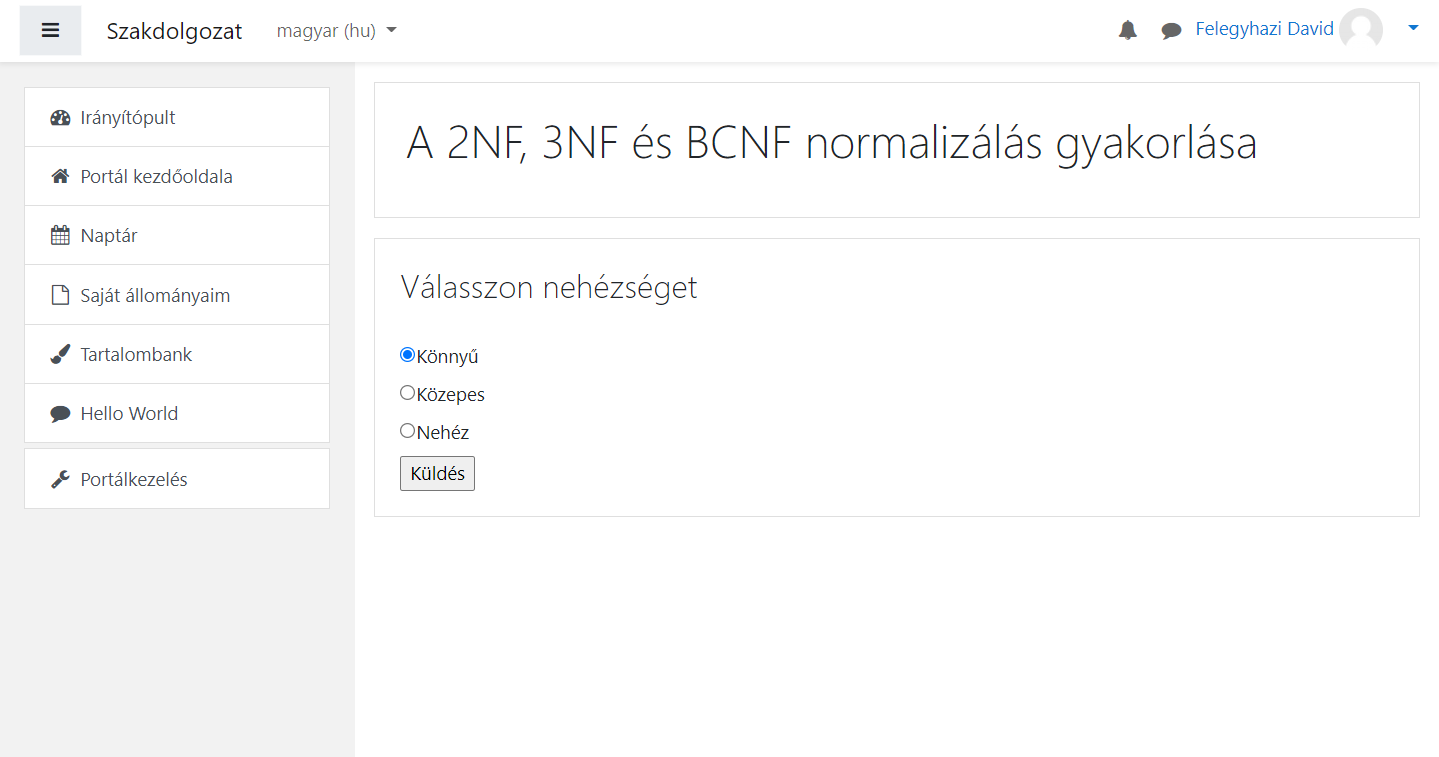
\includegraphics[scale=0.4]{Fejezetek/Images/magyar01.png}
    \caption{Nehézség kérése magyar nyelven}
\end{figure}
\begin{figure}
    \centering
    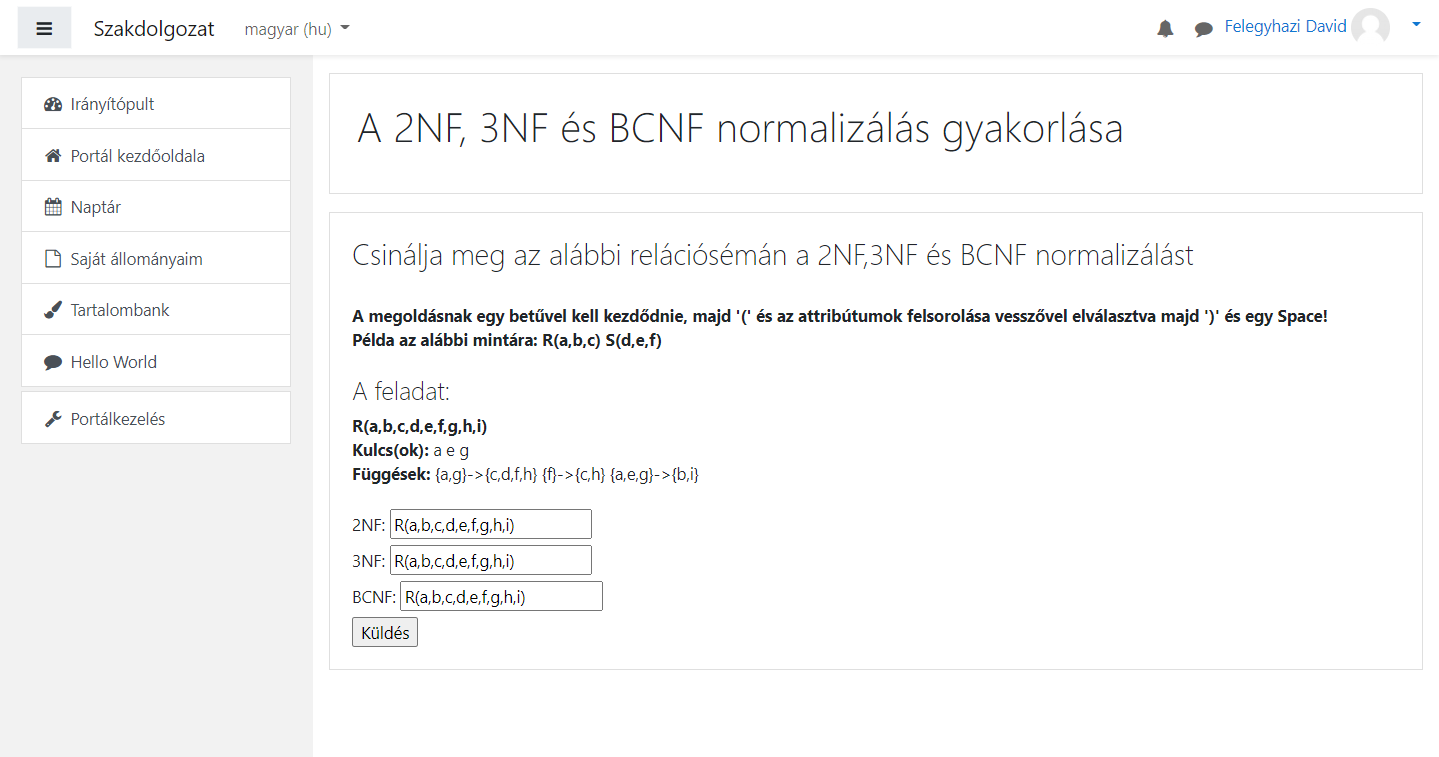
\includegraphics[scale=0.4]{Fejezetek/Images/magyar02.png}
    \caption{Feladat generálása és megoldás kérése magyar nyelven}
\end{figure}
\begin{figure}
    \centering
    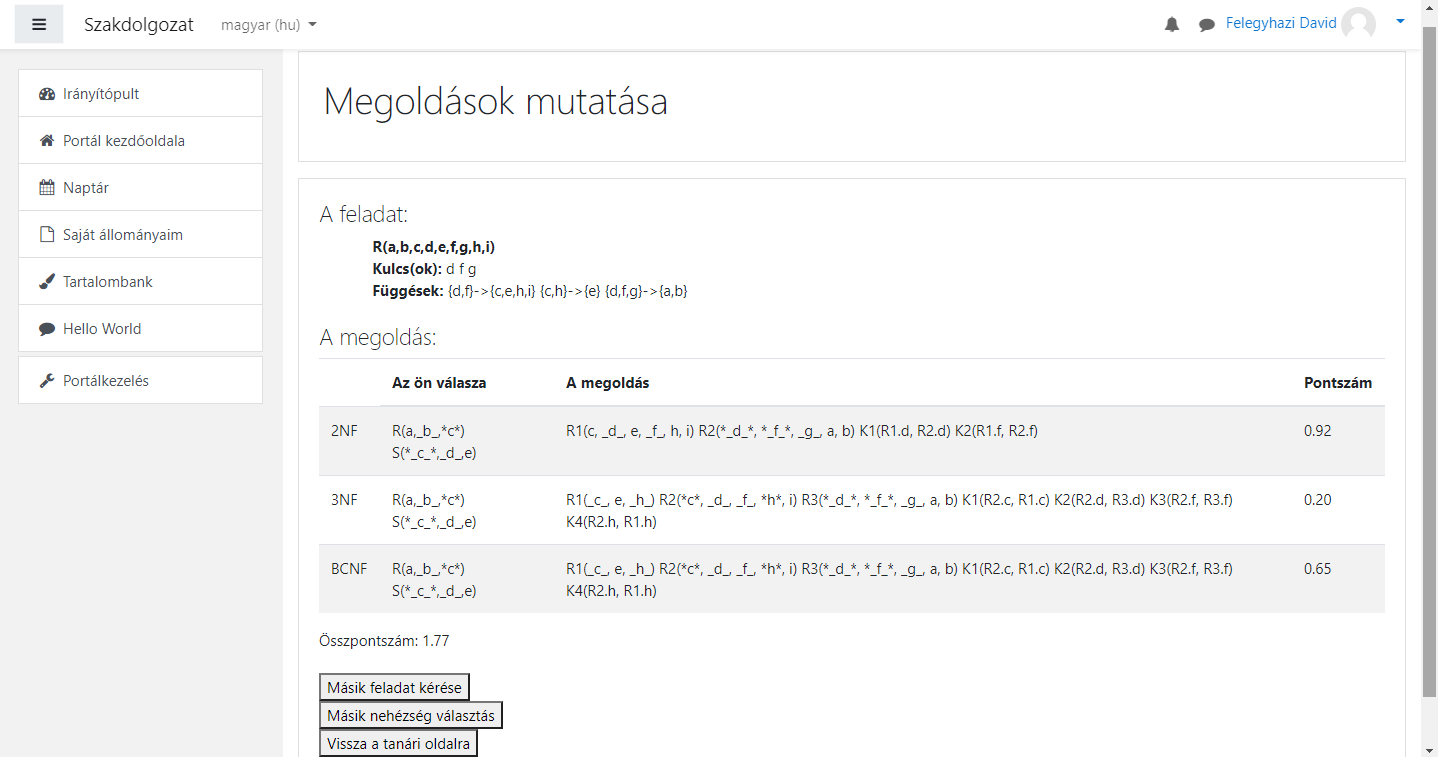
\includegraphics[scale=0.4]{Fejezetek/Images/magyar03.png}
    \caption{Megoldás mutatása a diák felületen magyar nyelven}
\end{figure}
\begin{figure}
    \centering
    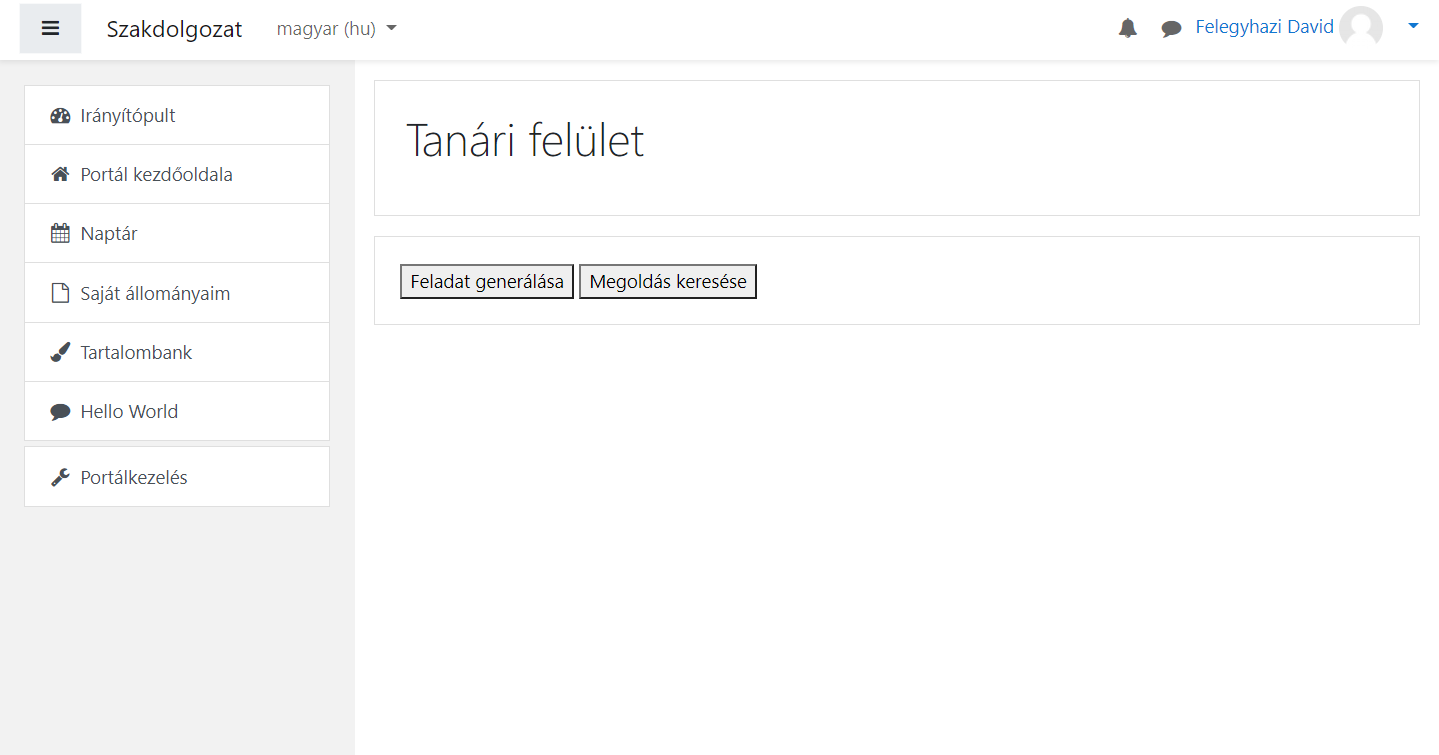
\includegraphics[scale=0.4]{Fejezetek/Images/magyar04.png}
    \caption{Megoldás mutatása a tanári felületen magyar nyelven}
\end{figure}
\begin{figure}
    \centering
    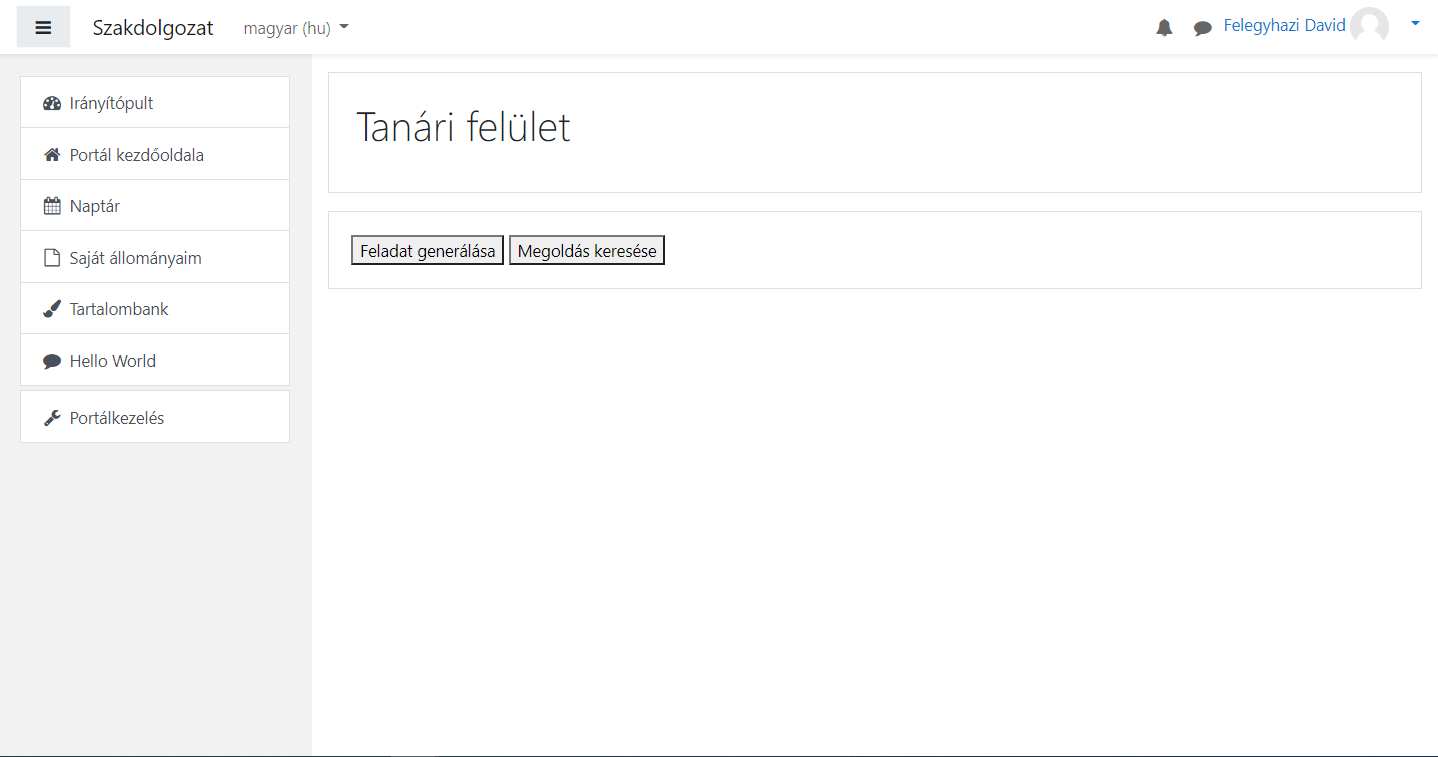
\includegraphics[scale=0.4]{Fejezetek/Images/magyar05.png}
    \caption{Tanári felület magyar nyelven}
\end{figure}
\begin{figure}
    \centering
    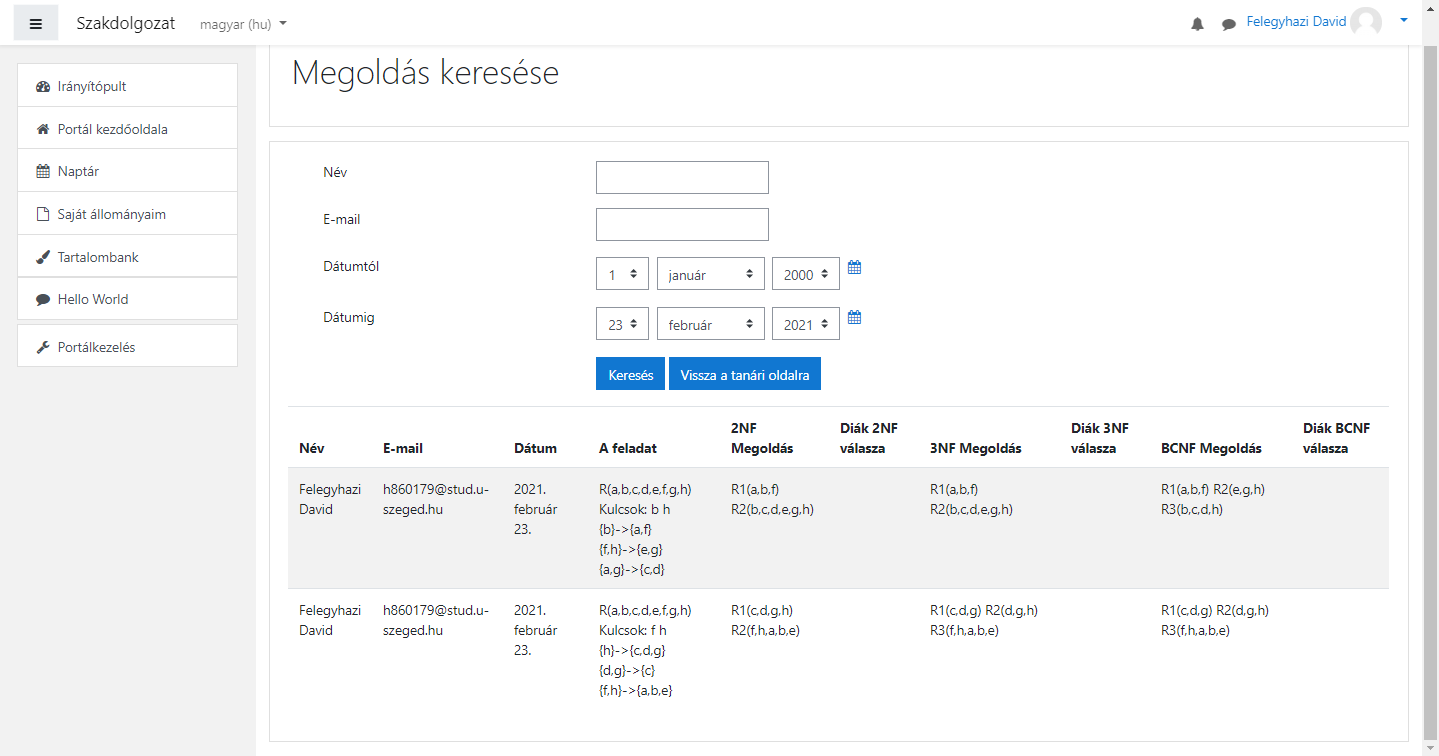
\includegraphics[scale=0.4]{Fejezetek/Images/magyar06.png}
    \caption{Keresőfelület magyar nyelven}
\end{figure}

\begin{figure}
    \centering
    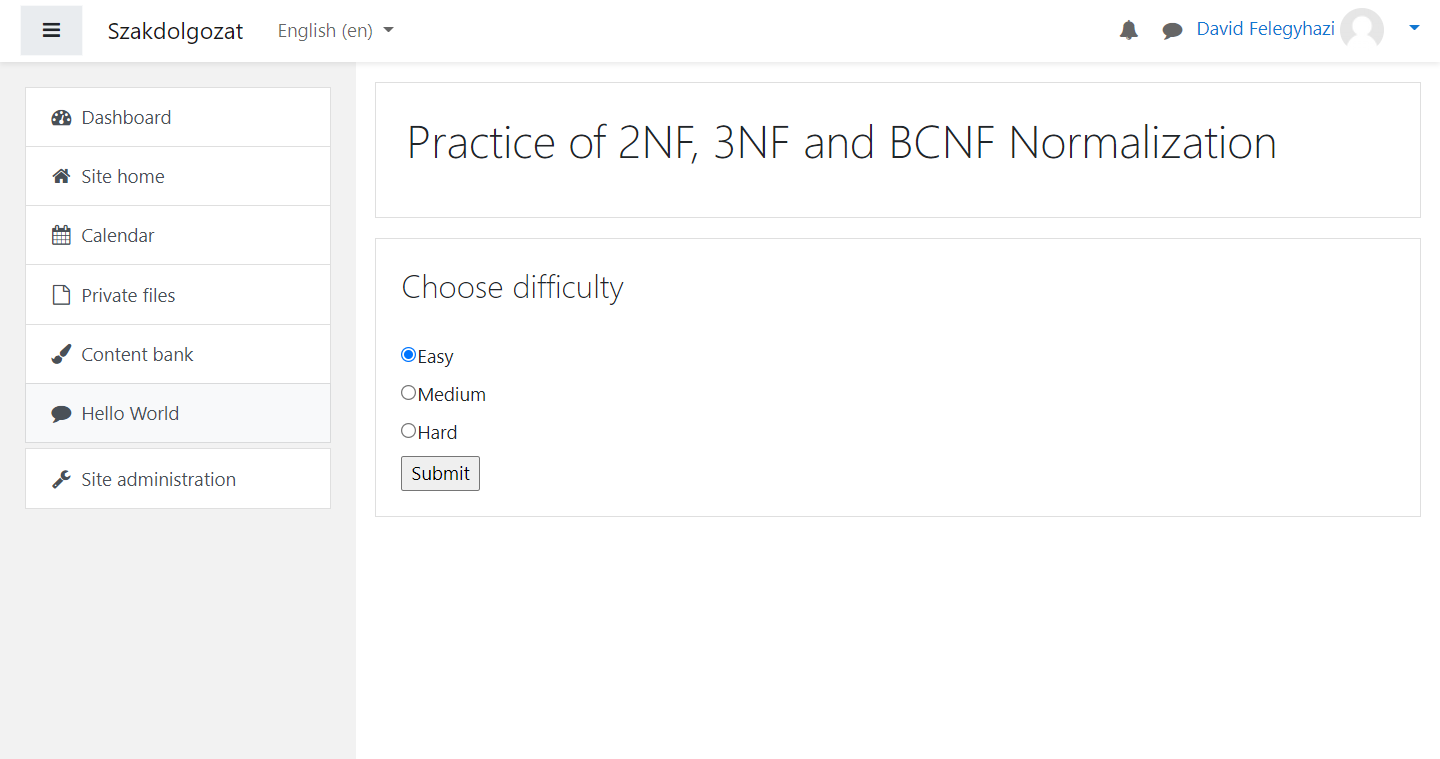
\includegraphics[scale=0.4]{Fejezetek/Images/english01.png}
    \caption{Nehézség kérése angol nyelven}
\end{figure}
\begin{figure}
    \centering
    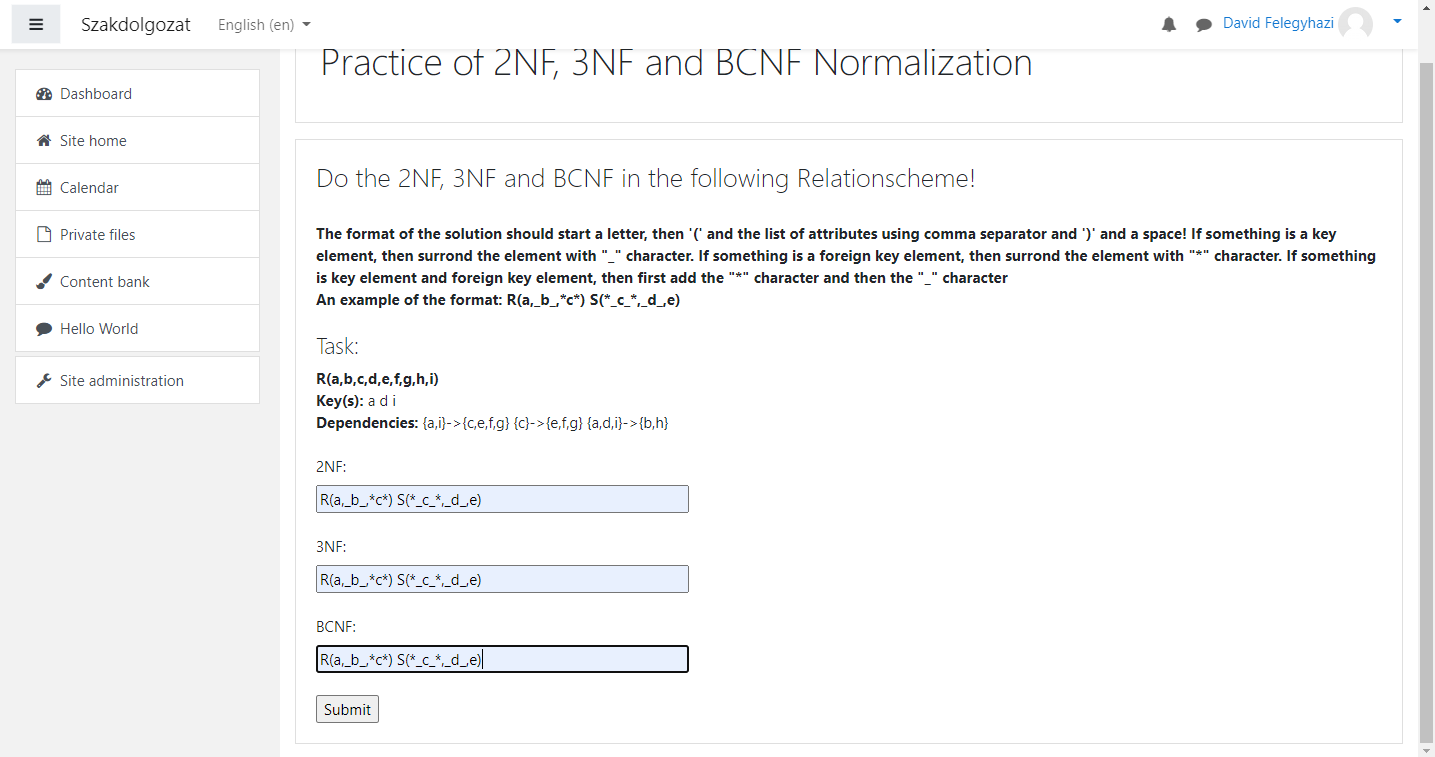
\includegraphics[scale=0.4]{Fejezetek/Images/english02.png}
    \caption{Feladat generálása és megoldás kérése angol nyelven}
\end{figure}
\begin{figure}
    \centering
    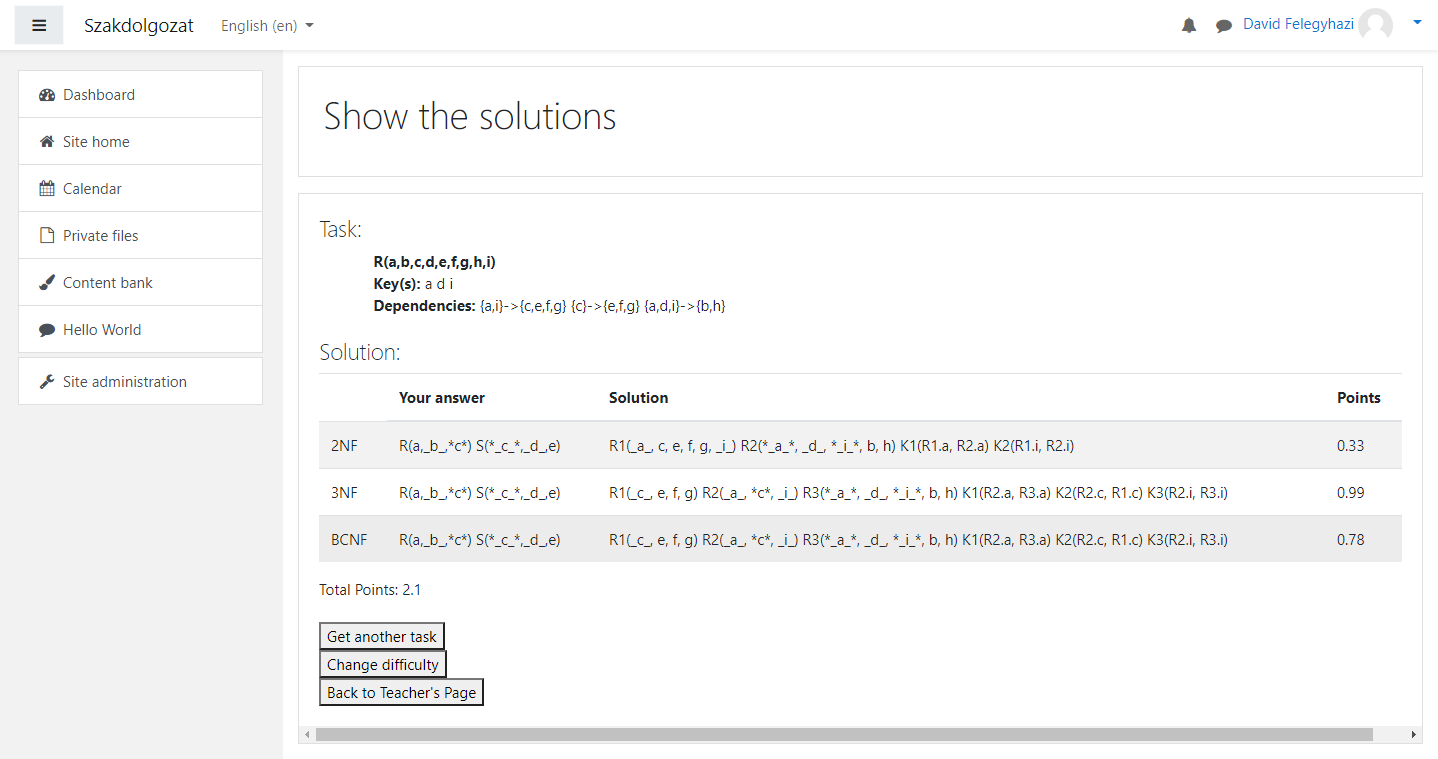
\includegraphics[scale=0.4]{Fejezetek/Images/english03.png}
    \caption{Megoldás mutatása a diák felületen angol nyelven}
\end{figure}
\begin{figure}
    \centering
    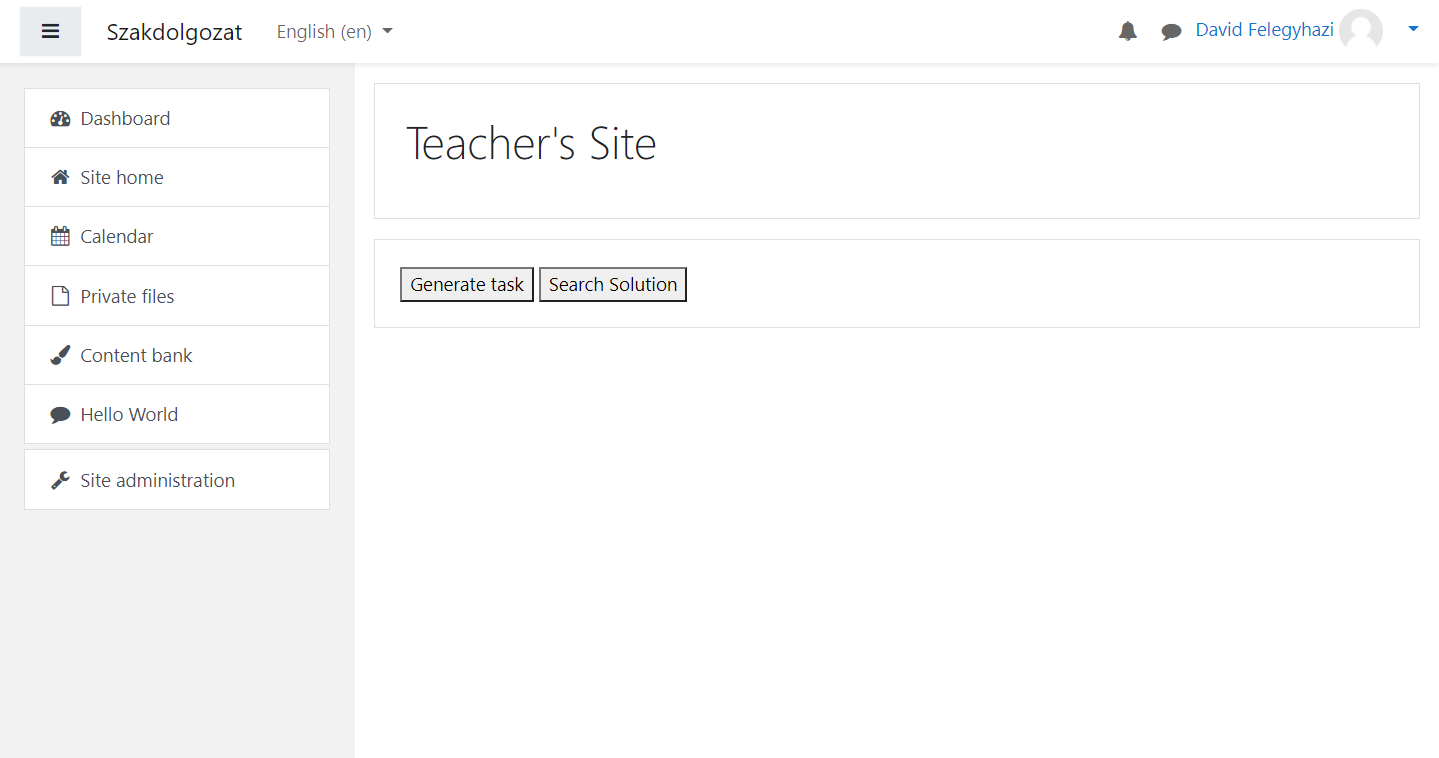
\includegraphics[scale=0.4]{Fejezetek/Images/english04.png}
    \caption{Megoldás mutatása a tanári felületen angol nyelven}
\end{figure}
\begin{figure}
    \centering
    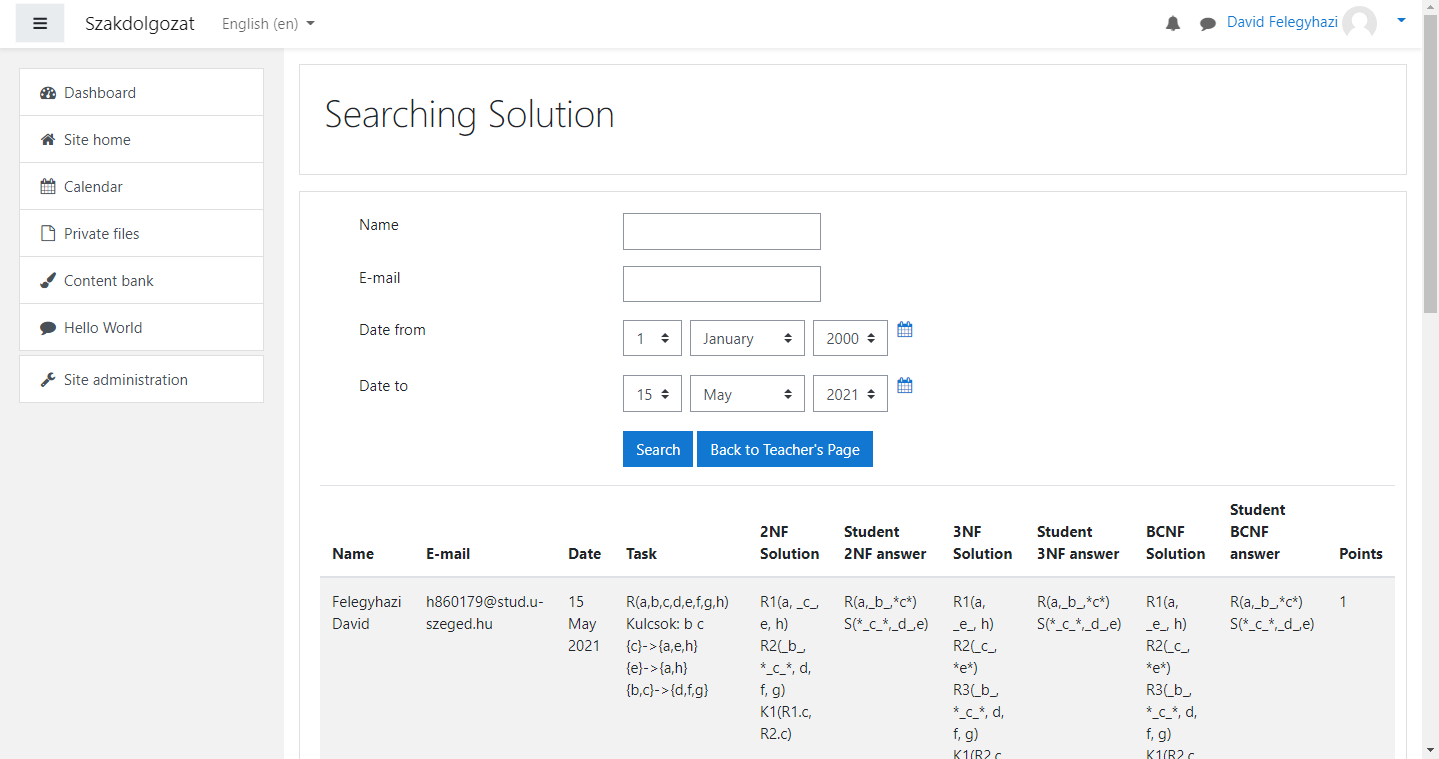
\includegraphics[scale=0.4]{Fejezetek/Images/english05.png}
    \caption{Tanári felület angol nyelven}
\end{figure}
\begin{figure}
    \centering
    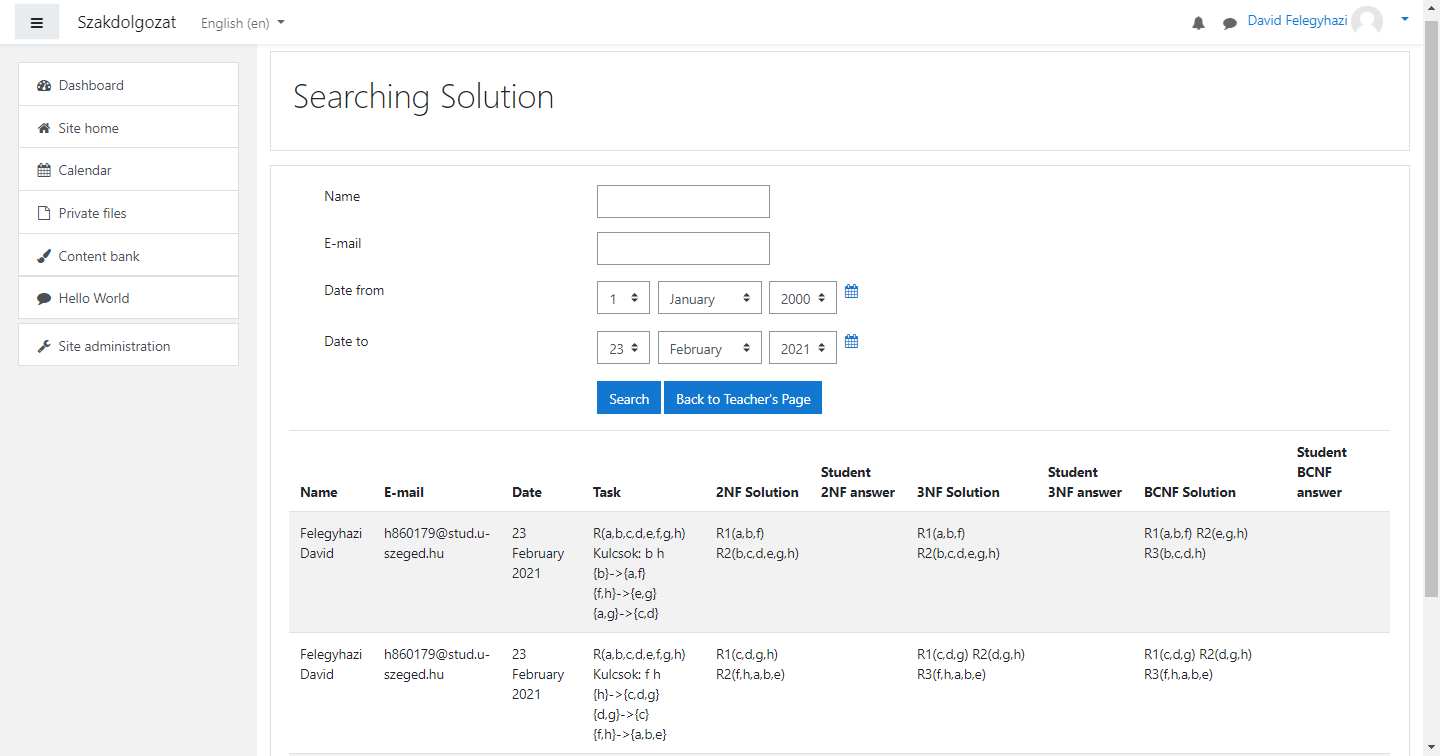
\includegraphics[scale=0.4]{Fejezetek/Images/englis06.png}
    \caption{Keresőfelület angol nyelven}
\end{figure}